\section{Tower: from Functions to Architectures}
\label{sec:tower}

\begin{figure*}[hbt!]
  \begin{tabular}{p{0.27\textwidth}|p{0.33\textwidth}|p{0.4\textwidth}}
    \begin{smcode}
blinkTower :: Tower ()
blinkTower = do
  (tx,rx) <- channel
  task "blink" (blinkTask tx)
  task "lightswitch" $
    onChannel rx $
      \textbackslash{}lit -> do
        ifte_ lit (turnOn light)
                  (turnOff light)
    \end{smcode}
&
    \begin{smcode}
blinkTask :: ChannelSource (Stored IBool)
      -> Task ()
blinkTask chan = do
  tx  <- withChannelEmitter chan
  res <- taskLocal
  onPeriod period $ \textbackslash{}now -> do
    res <- call blinkFromTime now
    emit_ tx res
  where period = Milliseconds 100
    \end{smcode}  %%$
&
    \raisebox{-\height}{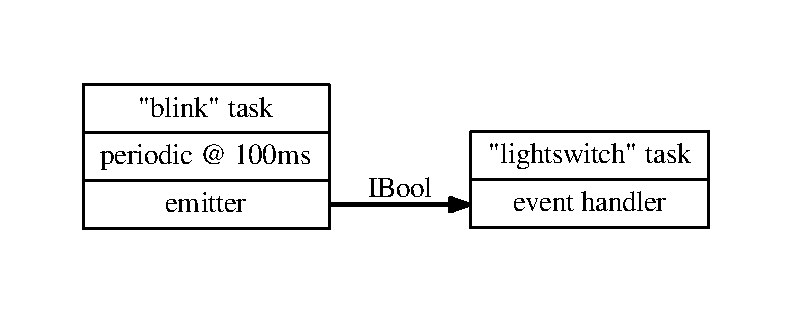
\includegraphics[width=6.5cm]{figures/tower-example}}
  \end{tabular}
  \caption{Tower (Col. 2), Task (Column. 1), Graphviz output (Col. 3)}
  \label{fig:tower-ex}
\end{figure*}


In many embedded systems, programmers produce an entire system of software
that interacts with multiple input and output peripherals concurrently using a
real-time operating system (RTOS). Typical RTOSes provide just a few low-level
locking and signaling primitives for scheduling. Since microcontrollers do not
have the virtual memory managment units (MMUs) found on larger processors, the
RTOS kernel cannot protect any system memory against badly behaved user code.
These restrictions put significant burden on programmers: they must ensure all
tasks, and all communication between tasks, are implemented correctly.

During our initial development of SMACCMPilot, we found ourselves writing
high-quality C functions in Ivory, which guarantees memory-safety of the
generated code. But whenever we needed
``glue code'' to implement inter-process communication, initialize
data-structures, read the system clock, lock the processor, etc., we were forced
to abandon our well-typed world and tediously use C directly via Ivory's foreign
function interface.  Furthermore, the hand-written C is OS-specific, meaning it
would have to be rewritten for any OS port.

\paragraph{Extending Ivory}
The hand-written glue code was ruining both our productivity and our assurance
story. We wanted a language to describe the structure of the glue code that
would generate it for us.
Our key insight was that such an EDSL could be built as a macro over Ivory,
using Ivory's code-generation facilities, without losing anything.

From these ideas, the Tower EDSL was born. You can think of Tower as an
extension to the Ivory language, designed to deal with the specific concerns of
multithreaded software architecture. Tower still allows the programmer to use
all the low-level power of Ivory for general programming, but uses a separate
language for describing tasks and the connections between them.  This is one of
the great productivity features of working with EDSLs: if you discover the
language you are using is difficult, tricky, or unsafe for solving a particular
problem, you can easily extend that language with a library without modifying
the compiler.

In Tower, one specifies tasks and communication channels, and the Tower compiler generate correct
Ivory implementations, as well as architecture description artifacts. Tower
hides the dangerous low-level scheduling primitives from the user, and keeps
type information for channels (i.e., the datatype of the channel message),
expressed as Ivory types, in the Haskell type system.

Tower allows the programmer to describe a static graph of channels and tasks.
For the intended use case in high assurance systems, a static configuration of
channels and tasks makes it easy to reason about memory requirements, and
permits the system to be analyzed for schedulability.

\paragraph{Multiple interpreters}

In the Tower front end, the programmer specifies a system that can be compiled
to multiple artifacts.

Tower is designed to support different operating systems via a swappable
backend. Since all code that touches operating system primitives is generated by
Tower, it is easy for the user to specify a system and compile it for
different operating systems. Tower supports both the open-soure
FreeRTOS\cite{freertos} as well as the formally-verified
eChronos RTOS\cite{echronos} developed by NICTA.

Tower also has a backend which generates a system description in the Architecture
Analysis and Design Language (AADL)~\cite{SAE:AADL}. We also built a backend for
the Graphviz dot language.  These output formats make it possible to visualize,
analyze, and automatically check properties about the system.

We were pleased by the productivity improvements and correctness guarantees the
Tower language provided. In all, it took about 4 engineer-months to build Tower,
and a total of about 3000 lines of Haskell code.


\paragraph{Tower example}
\label{sec:examples}

In Figure~\ref{fig:tower-ex}, we sketch a small Tower example that is
representative of a device driver that blinks an LED.  Small simplifications to
Tower have been made in the code, eliding details relating to code generation
and backend selection.

In the first column of the figure, the communication
architecture is defined in the \cd{Tower} monad.  The program initializes a
unidirectional channel between two tasks as well as the tasks themselves.  A channel, or queue,
consists of transmit (\cd{tx}) and receive (\cd{rx}) endpoints, respectively.
The \cd{blinkTask} task is an RTOS task that will send output to the
\cd{lightswitch} RTOS task via an RTOS-mediated channel.  The \cd{lightswitch}
task toggles the LED based on the incoming Boolean values.  (In the third column, a graph of the tower program is shown, generated from the
Tower compiler's Graphviz dot output, showing the architectural structure of the
two tasks as well as the queue between them.)

To conserve space, we only define \cd{blinkTask}.  The second column contains
the definition of \cd{blinkTask}, defined in the \cd{Task} monad.  The
\cd{blinkTask} task takes a channel source and returns a task.  The
task first initializes an \emph{emitter} for the channel then creates a
reference to allocated memory that is private to the task.  Every 100
milliseconds, an Ivory action is taken.  In this case, the action is to call
Ivory function \cd{blinkfromTime} that is executed whenever the task is enabled
(we elide the implementation of \cd{blinkfromTime} in this example).  The
boolean value \cd{res} is then emitted on the channel.


%% . The \cd{blinkTask} task is has fields for
%% properties and communications ports, showing its periodic rate and emitter. The
%% \cd{lightswitch} task only has one port, the event handler created by the
%% \cd{onChannel} primitive. A channel, annotated with its Ivory datatype
%% \cd{IBool}, is shown as a directed graph edge connecting from \cd{blinkTask}'s
%% emitter to \cd{lightswitch}'s event handler.


